\chapter{Comunicazione tra i Nodi e il Sink}
  \section{Descrizione del Problema}
    L'architettura presentata è stata sviluppata con l'obiettivo di gestire un alto grado di asincronismo tra le varie parti del sistema. L'istante di trasmissione dei dati, infatti, è imprevedibile e può avvenire in qualsiasi momento, ciò è dovuto al fatto che l'arrivo dei dati sui nodi non è periodico e, di conseguenza, anche la creazione del relativo modello. Tutto ciò rende imprevedibile anche l'istante in cui i modelli vengono unificati dal Sink, il quale necessita dei modelli di tutti i nodi per effettuare il \textit{Merging}.  \newline

    Per rispettare questi requisiti è necessario addottare tecniche di comunicazioni asincrone, in grado di gestire la trasmissione e l'arrivo dei dati in un qualunque istante nel tempo. Un protocollo che si presta bene a queste esigenze è il Protocollo \textbf{AMQP} (\textit{Advanced Message Queueing Protocol}), il quale garantisce funzionalità di messaggistica, accodamento, routing ( con paradigmi Point-to-Point e Public\&Subscribe). \newline

    Nel caso considerato, la comunicazione è bidirezionale in quanto da un lato i nodi inviano i modelli locali al Sink, dall'altro il Sink invia il modello Unificato a tutti i nodi, i quali aggiornano il proprio modello locale con quello Unificato, se considerato più accurato. Visto che entrambe le parti interpretano il ruolo sia di mittente che di destinatario, si è scelto di gestire le due comunicazioni con tecniche differenti, come spiegato nei paragrafi seguenti.
    \subsection{Comunicazione da Nodo a Sink}
      Un modello è prodotto da un Nodo (\textit{Producer}) e inviato al Sink (\textit{Consumer}), che rappresenta l'unico ricevitore. In uno scenario del genere è sufficiente adottare una communicazione del tipo mostrata in figura \ref{fig:ProducerConsumer} nella quale un produttore invia i propri dati sulla coda, successivamente consumati dal consumatore. Questa tipologia di comunicazione è usata da ogni Nodo, quindi, dal punto di vista del Sink, ci saranno \textit{N} produttori che riempiranno la sua coda.
      \begin{figure}[h!]
        \centering
        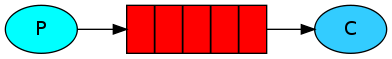
\includegraphics[scale=0.7]{../Immagini/ProducerConsumer.png}
        \caption{Comunicazione con un Producer e un Consumer}
        \label{fig:ProducerConsumer}
      \end{figure}

    \subsection{Comunicazione da Sink a Nodo}
      Il Sink produce il modello Unificato che deve essere distribuito all'intera pool di Nodi. Il paradigma di comunicazione migliore da seguire in questo caso è quello del \textit{Public\&Subscribe}, rappresentato in figura \ref{fig:PublicSubscribe}. Tramite questo paradigma il Sink comunica ad un \textit{Exchange} ( il nodo in blu della figura ) il modello e questo lo posta su ogni coda di ogni consumatore ( i Nodi ).
      \begin{figure}[h!]
        \centering
        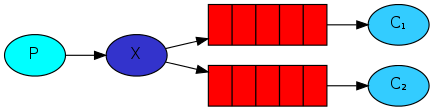
\includegraphics[scale=0.7]{../Immagini/PublicSubscribe.png}
        \caption{Comunicazione Public\&Subscribe}
        \label{fig:PublicSubscribe}
      \end{figure}

    \subsection{Registrazione di un nuovo Nodo}
      Per rendere l'architettura dinamica e flessibile è stato sviluppato un meccanismo per incrementare o diminuire il numero dei Nodi nel sistema. A questo scopo, quando un nodo vuole unirsi alla pool, deve necessariamente informare il Sink in modo tale che quest'ultimo tenga costantemente traccia del numero di Nodi presenti, necessario per l'operazione di Merging dei modelli. \newline
      La soluzione migliore in questo caso è quella di sfruttare un sistema di \textbf{RPC} (\textit{Remote Procedure Call}) che permette al Nodo di effettuare delle chiamate di funzioni eseguite sul Sink. Come mostrato in figura \ref{fig:RPC}, questo meccanismo si compone di 2 code:
      \begin{itemize}
        \item \textit{rpc\_queue}: coda delle chiamate di funzioni
        \item \textit{reply\_to}: coda dei risultati delle funzioni
      \end{itemize}
      Nel caso considerato, le funzioni disponibili sono le seguenti:
      \begin{itemize}
        \item \textit{Registration}: un nodo richiede l'accesso alla pool e ottiene un identificativo univoco come risposta
        \item \textit{Leave}: un nodo richiede l'uscita dalla pool specificando il proprio identificativo nella richiesta
      \end{itemize}
      \begin{figure}[h!]
        \centering
        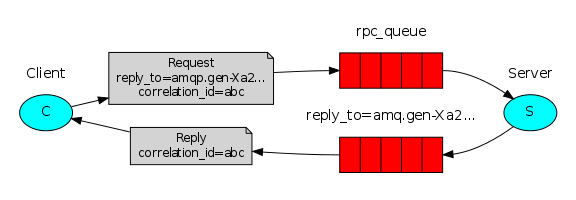
\includegraphics[scale=0.7]{../Immagini/RPC.png}
        \caption{Remote Procedure Call}
        \label{fig:RPC}
      \end{figure}


  \section{Implementazione}
    \subsection{abstract class CommunicationModelHandler}
      Il software creato si appoggia sulle Java API di \textit{RabbitMQ} che permette una facile gestione di message queueing e per via delle somiglianza tra le azioni da svolgere sia sul Sink che sui Nodi, è stata implementata una classe astratta \textit{CommunicationModelHandler} \ref{CommunicationHandler} che mantiene delle informazioni utilizzati nelle interazioni con il server di RabbitMQ e i nomi delle \textit{Queue}, comuni a tutti i nodi. Inoltre, il costruttore inizializza una connessione con il Server di RabbitMQ configurato sulla porta di default 5672 e richiama le 3 funzioni per l'inizializzazione delle strutture su cui verrano scambiati i dati:
      \begin{itemize}
        \item \textit{initRPC()}
        \item \textit{initSinkToNode()}
        \item \textit{initNodeToSink()}
      \end{itemize}
      Ognuna di queste verrà definita dal Nodo e dal Sink in modo da rispettare il proprio ruolo rispetto alla struttura in questione.
      \lstinputlisting[label={CommunicationHandler}, language=Java, caption={CommunicationModelHandler},captionpos=b]{../Codice/CommunicationModelHandler.java}

    \subsection{NodeCommunicationModelHandler}
      Questa classe è l'implementazione della \textit{CommunicationModelHandler} utilizzata su ogni Nodo per la gestione della communicazione con il Sink. Ai campi membri della super classe viene aggiunto un intero \textit{NodeID} che contiene l'identificativo del nodo. La classe definisce le funzioni astratte nel seguente modo:
      \subsubsection{initRPC()}
        Questa funzione crea un canale per comunicare con il Server RPC presente sul Sink attraverso cui si chiama la Remote Procedure per <<registrare>> il Nodo nel sistema, il quale ottiene un identificativo univoco come risposta. Tale ID è usato per distinguere i nodi tra di loro e i loro relativi modelli.
        \lstinputlisting[label={Node:initRPC}, language=Java, firstline=32, lastline=43,  caption={NodeCommunicationModelHandler.initRPC()},captionpos=b]{../Codice/NodeCommunicationModelHandler.java}

      \subsubsection{initNodeToSink()}
        \'E sufficiente dichiarare sul canale opportuno la coda del Sink sulla quale riceve i modelli, nominata \textbf{NODE\_TO\_SINK\_QUEUE}, di tipo:
        \begin{itemize}
          \item non \textit{durable}: la coda non sopravvive ad un restart del server
          \item non \textit{exclusive}: non ristretta a questa connessione
          \item non \textit{autoDelete}: il server non cancellerà la coda se non più in uso
        \end{itemize}
        \lstinputlisting[label={Node:initNodeToSink}, language=Java, firstline=44, lastline=54,  caption={NodeCommunicationModelHandler.initNodeToSink()},captionpos=b]{../Codice/NodeCommunicationModelHandler.java}

      \subsubsection{initSinkToNode()}
        In questo caso bisogna legare il nodo all'\textit{Exchange} del Sink in modo da ricevere qualsiasi modello Unificato da esso prodotto. A questo scopo, si dichiara l'Exchange di nome \textbf{SINK\_TO\_NODE\_EXCHANGE} di tipo \textit{fanout}, che effettua il broadcast di tutti i messaggi che riceve a tutte le code che conosce, e da questo si ottiene una coda temporanea sulla quale il nodo riceve i messaggi. Eseguendo la \textit{basicConsume(...)} il nodo inizia ad ascoltare i messaggi sulla coda che vengono processati dal \textit{Consumer ModelReceiver} di cui si parla in \ref{ModelReceiver}.
        \lstinputlisting[label={Node:initSinkToNode}, language=Java, firstline=55, lastline=73,  caption={NodeCommunicationModelHandler.initSinkToNode()},captionpos=b]{../Codice/NodeCommunicationModelHandler.java}

      \subsubsection{receiveModel(Model deliveredModel)}
        Alla ricezione di un nuovo modello Unificato, il nodo deve comunicare al modulo del Machine Learning che è necessario valutare l'aggiornamento del modello locale con quello appena ricevuto. Si contatta il server Rest con il comando \textit{Update}, specificando inoltre l'ID del nodo, attivando un thread apposito per evitare attese attive sulla risposta del server Rest.
        \lstinputlisting[label={Node:receiveModel}, language=Java, firstline=74, lastline=89,  caption={NodeCommunicationModelHandler.receiveModel()},captionpos=b]{../Codice/NodeCommunicationModelHandler.java}

      \subsubsection{sendModel()}
        Per inviare un modello al Sink è sufficiente leggerlo dal file creato dal modulo di ML ed effettuare la funzione \textit{basicPublish(...)} specificando la coda in cui inserire il modello e i byte da inviare.
        \lstinputlisting[label={Node:sendModel}, language=Java, firstline=90, lastline=99,  caption={NodeCommunicationModelHandler.sendModel()},captionpos=b]{../Codice/NodeCommunicationModelHandler.java}

    \subsection{SinkCommunicationModelHandler}
      Questa classe è un'estensione della \textit{CommunicationModelHandler} utilizzata dal Sink per la gestione della comunicazione con i Nodi. Ai campi membri della super classe, si aggiungono:
      \begin{itemize}
        \item \textit{int nextID}: un intero incrementale che indica l'ID da assegnare al prossimo nodo che si unisce al sistema
        \item \textit{HashMap<Integer,Boolean>} isNew: che permette di verificare se il Sink ha ricevuto un modello fresco da un determinato nodo
        \item \textit{boolean merging}: indica se è in corso il merging o meno
      \end{itemize}

      \subsubsection{initRPC()}
        Avvia il thread relativo a \textit{RPCServer} di cui si parla in \ref{RPCServer}.
        \lstinputlisting[label={Sink:initRPC}, language=Java, firstline=51, lastline=55,  caption={SinkCommunicationModelHandler.initRPC()},captionpos=b]{../Codice/SinkCommunicationModelHandler.java}

      \subsubsection{initNodeToSink()}
        Si dichiara una coda come in \ref{Node:initNodeToSink} ma questa volta si esegue la \textit{basicConsume(...)} per stare in ascolto dei modelli inviati dai nodi
        \lstinputlisting[label={Sink:initNodeToSink}, language=Java, firstline=26, lastline=39, caption={SinkCommunicationModelHandler.initNodeToSink()},captionpos=b]{../Codice/SinkCommunicationModelHandler.java}

      \subsubsection{initSinkToNode()}
        Si dichiara l'\textit{Exchange} come in \ref{Node:initSinkToNode}, tuttavia senza avviare il consumo dei messaggi.
        \lstinputlisting[label={Sink:initSinkToNode}, language=Java, firstline=40, lastline=50, caption={SinkCommunicationModelHandler.initSinkToNode()},captionpos=b]{../Codice/SinkCommunicationModelHandler.java}

      \subsubsection{receiveModel(Model deliveredModel)}
        Alla ricezione di un nuovo modello questo viene conservato in 2 file:
        \begin{itemize}
          \item \textit{dataSink/ModelNodeID.json} dove ID indica l'id del nodo che ha inviato il modello
          \item \textit{dataSink/history/Node-ID/} e come nome del file si usa il timestamp di ricezione del modello. In questa cartella è conservato uno storico dei modelli inviati da nodo con quel determinato ID.
        \end{itemize}
        Si aggiorna la freschezza del modello nella mappa isNew e si controlla se avviare il processo di merging o meno, avviato solo se i modelli di tutti i nodi risultano essere freschi e se non vi è un merging già in corso. In caso positivo, si avvia il thread \textit{ModelMerger} di cui si parla in \ref{ModelMerger}.
        \lstinputlisting[label={Sink:receiveModel}, language=Java, firstline=56, lastline=68, caption={SinkCommunicationModelHandler.receiveModel(...)},captionpos=b]{../Codice/SinkCommunicationModelHandler.java}

      \subsubsection{sendModel()}
        Legge il modello Unificato creato dal modulo ML e lo pubblica sull'\textit{Exchange} \textbf{SINK\_TO\_NODE\_EXCHANGE}, resetta la freschezza di tutti i modelli nella mappa isNew e dichiara concluso il merging.
        \lstinputlisting[label={Sink:sendModel}, language=Java, firstline=69, lastline=82, caption={SinkCommunicationModelHandler.sendModel()},captionpos=b]{../Codice/SinkCommunicationModelHandler.java}

      \subsubsection{registration()}
        Funzione chiamata da RPCServer quando quest'ultimo riceve una richiesta di registrazione da un nodo. La risposta alla richiesta contiene il valore ritornato da questa funzione, corrispondente all'ID assegnato al nodo entrante.
        \lstinputlisting[label={Sink:registration}, language=Java, firstline=89, lastline=96, caption={SinkCommunicationModelHandler.registration()},captionpos=b]{../Codice/SinkCommunicationModelHandler.java}

      \subsubsection{removeNode(int nodeID)}
        Funzione chiamata da RPCServer quando riceve una richiesta di uscita dal sistema dal nodo. Rimuove il nodo con l'ID specificato dalla mappa isNew e ritorna \textbf{OK} se l'operazione è avvenuta con successo, altrimenti \textbf{NOT FOUND}.
        \lstinputlisting[label={Sink:removeNode}, language=Java, firstline=97, lastline=106, caption={SinkCommunicationModelHandler.removeNode()},captionpos=b]{../Codice/SinkCommunicationModelHandler.java}

    \subsection{ModelMerger}\label{ModelMerger}
      Effettua una richiesta al server Rest con il comando \textit{Merge} e sta in attesa della risposta. La risposta può contenere i seguenti codici:
      \begin{itemize}
        \item 201: il modello è stato unificato con successo, quindi è possibile inviarlo ai nodi tramite la \textit{SinkCommunicationModelHandler.sendModel()}
        \item 204: attualmente esiste solo un modello, quindi è inutile effettuare il merging
        \item 500: si è verificato un errore nel modulo ML
        \item altrimenti: codice non supportato
      \end{itemize}
      \lstinputlisting[language=Java, firstline=8, lastline=41, caption={ModelMerger},captionpos=b]{../Codice/ModelMerger.java}

    \subsection{RPCServer}\label{RPCServer}
      RPCServer è un thread che sta continuamente in ascolto di richeste dei nodi in arrivo sulla coda \textbf{RPC\_NODE\_TO\_SINK\_QUEUE\_NAME}. Le richieste vengono processate dal \textit{DeliverCallback}, definito nella funzione run del thread, che richiama l'oppurtuna funzione del Sink ( \ref{Sink:registration} oppure \ref{Sink:removeNode} ) e risponde alla richiesta tramite la \textit{basicPublish(...)}.
      \lstinputlisting[language=Java, firstline=14, lastline=87, caption={ModelMerger},captionpos=b]{../Codice/RPCServer.java}

    \subsection{Classi comuni tra Nodo e Sink}
      \subsubsection{Model}
        Contiene l'ID del nodo che ha generato il modello e una stringa che contiene la rappresentazione json del modello. In caso in cui il modello sia quello unificato prodotto dal Sink, il nodeID contiene -1.
        \lstinputlisting[language=Java, firstline=6, caption={Model},captionpos=b]{../Codice/Model.java}

      \subsubsection{ModelReceiver}\label{ModelReceiver}
        Questa classe implementa l'interfaccia Consumer di RabbitMQ e permette di definire le azioni da compiere in base all'evento ricevuto. In particolare, alla ricezione di un nuovo modello, viene chiamata la funzione \textit{receiveModel} del relativo \textit{CommunicationModelHandler}.
        \lstinputlisting[language=Java, firstline=10, caption={ModelReceiver},captionpos=b]{../Codice/ModelReceiver.java}

      \subsubsection{Config}
        Classe che contiene le varie costanti usate nel progetto.
        \lstinputlisting[language=Java, firstline=6, caption={Config},captionpos=b]{../Codice/Config.java}
